\begin{figure}[t]
\centering
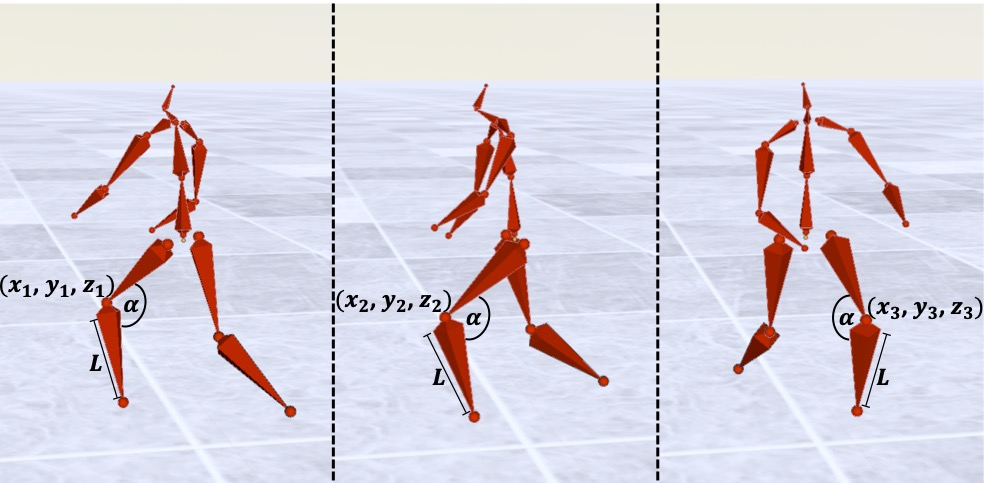
\includegraphics[width=0.9\linewidth]{./images/Skeleton_angles.pdf}
\caption{Human rigs observed via the relative axis systems of three cameras. 3D locations vary across axis systems while 3D rotation angles (illustrated with a 2D symbol) and bone lengths remain identical. Thus, fusing the former requires acquaintance of camera parameters while fusing the latter requires none. }
\label{fig:skeleton_angles}
\end{figure}